\chapter{Methodology}
This chapter will describe the workflow, and a detailed explanation of our implementation. At the end of this chapter we will discuss the testing of our implementation.
\section{Workflow and project structure}
The code were mostly written in Emacs on Ubuntu 14.04 LTS running in VirtualBox on a Windows8.1 laptop. Git was used to transfer files between the virtual machine and other computers used write code.

The file structure is shown in \ref{code:structure}. 
\begin{lstlisting}[caption={Project structure}, label={code:structure}]
|-- buttons.h
|-- core
|-- dac.c
|-- efm32gg.h
|-- ex2.bin
|-- ex2.c
|-- gpio.c
|-- interrupt_handlers.c
|-- lib
|   |-- efm32gg.ld
|   |-- ex2.bin
|   |-- libefm32gg.a
|-- Makefile
|-- songs.h
|-- timer.c
|-- tone-generator.py
|-- tones.h
\end{lstlisting}

\subsubsection{Header files}
All the header files are used to store predefined variables. efm32gg.h contains memory locations for the most used registers. 
tones.h contains implementation specific values for the different tones used, explained further in section \ref{sec:generating}. 
songs.h contains a struct, defining how we store songs, and also contains the songs and sound effects used in this exercise.
buttons.h contains the register values on different key presses, for easy comparison on GPIO interrupt.

\subsubsection{C-Files}
ex2.c is the main file, which is run at power-on. 
gpio.c, timer.c and dac.c has code for setting up and powering on and off the different parts.
interrupt_handlers.c contains the code for handling interrupts, which is also the code that actually plays the sound.

\subsection{Bulding and flashing}
\label{sec:bulding}
The GNU-Toolchain was used to compile and build the C-code. This was done using the \texttt{make} command. The binary was then uploaded to the board, via USB, using Silicon Labs' eACommander.

\subsection{Debugging}
We were not able to install the gdb tool for ARM on the virtual machine. This made debugging quite hard, and lead to a try and fail approach. If we needed to know the value of a variable or a register, we wrote the binary value to the gamepad's LEDs.

\section{Implementation}
To get started, and to get familiar with programing a microcontroller using the C language, we reimplemented the functionality of Exercise 1 \cite{ex1}. This included the setup of GPIO, clocks and interrupts.

\subsection{Setting Up}
To make thing work, we need to run some initial code to set things up. 
\subsubsection{GPIO}
To make the General-Purpose-Input-Output work, we first enable the GPIO clock by setting a value to the CMU register.
Then we enable high drive strength and set pin 8 to 15 as output, on Port A, for the gamepad's LEDs. We also need to make the buttons work, which is done by writing some values to GPIO\_PA registers.
Finally we enable interrupt on button presses.

\subsubsection{DAC}
Next we set up the DAC. We need the high peripheral clock to drive this as well. So we write to to bit number 17 in CMU\_HFPERCLKEN0. We want sound in both left and right speaker, so DAC0\_CH0CTRL and DAC0\_CH0CTRL is set to 1.

\subsubsection{Timer}
\label{sec:timer}
The timer is also driven by the high peripheral clock. Bit 6 is set to enable this. After this, TIMER1\_TOP is set to 140. This will make the timer count to 140, and then restart at 0. We enable interrupt on this event.

\subsubsection{NVIC}
The Nested Vector Interrupt Controller handles the interrupts from the different components on the board. In this implementation we need to handle interrupts from three different sources; GPIO\_ODD, GPIO\_EVEN and TIMER1. To do this we simply write 1 to their respecive bits in the ISER0 register found in \citep{interrupt}

\subsection{Generating sound}
\label{sec:generating}
Our next goal was to get a simple tone playing. As explained in section \ref{sec:dac} sound is moving air. To get the 440Hz tone we wanted, we need to change the value in the DAC 880 times per second. This makes a square pulse with a period of 440Hz.
To make this happen, we made use of the timer explained in section
\ref{sec:timer}. We sat TIMER1\_TOP to 140, as mentioned in \ref{sec:timer}, which gave us 100000 interrupts per second. This is because the clock that drives the timer runs at 14Mhz.

\begin{center}
$14000000Hz/140=100000Hz$
\end{center}

In the interrupt handler we used two counters. One to keep track of when to feed a new value to the DAC, and one for when to change the tone.
We used a tone generator script written in python \ref{app:py} to generate a header file with the values for each tone. These values indicates how many interrupts there should be between each time we feed a new value to the DAC.

Since we use square waves, there is no need to sample a sine wave and feed different values to the DAC. We simply write voltage/no-voltage. The voltage is defined is a volume variable, which is XORed to the DAC at every half period. 

\subsubsection{}

\subsection{Improvements}

\subsubsection{}

\section{Testing}
Add content in this section that describes how you tested and verified the correctness of your implementation, with respect to the requirements of the assignment.
\begin{figure}
\centering
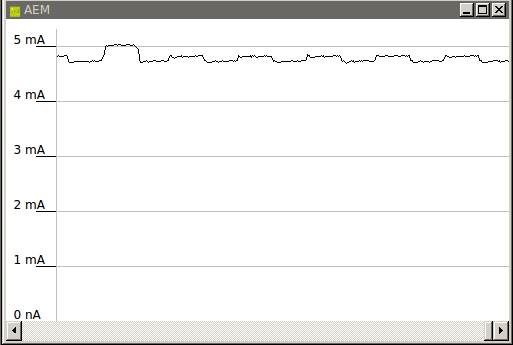
\includegraphics[scale=1]{images/Idle_preEF.PNG}
\caption{A JPEG image of a galaxy. Use vector graphics instead if you can.}
\label{fig:universe}
\end{figure}